\documentclass{article}
\usepackage{amsmath}
\usepackage{amssymb}
\usepackage{pgfplots}
\pgfplotsset{compat=1.16}

\begin{document}

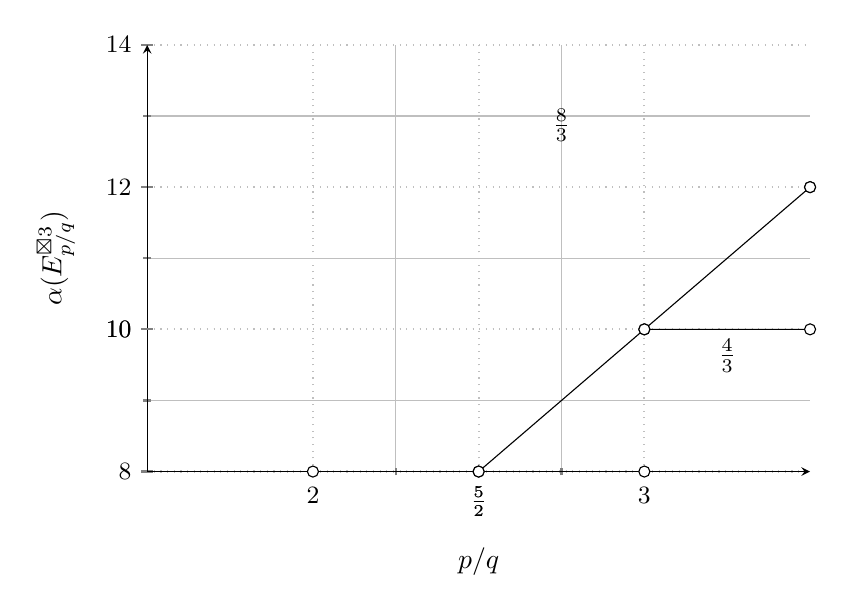
\begin{tikzpicture}
    \begin{axis}[
        axis lines=left,
        xlabel=$p/q$,
        ylabel=$\alpha(E_{p/q}^{\boxtimes 3})$,
        xmin=1.5, xmax=3.5,
        ymin=8, ymax=14,
        xtick={2, 2.5, 3},
        ytick={8, 10, 12, 14},
        yticklabels={8, 10, 12, 14},
        xticklabels={2, $\frac{5}{2}$, 3},
        extra x ticks={5/2},
        extra x tick labels={$\frac{5}{2}$},
        extra y ticks={10},
        extra y tick labels={$10$},
        extra y tick style={grid=major},
        extra x tick style={grid=major},
        every tick/.append style={thick},
        grid=both,
        major grid style={dotted, thick},
        minor tick num=1,
        tick label style={font=\small},
        width=10cm,
        height=7cm,
    ]
    
    % Plotting the step function
    \addplot[mark options={fill=white}, mark=*] coordinates {
        (2, 8) (2.5, 8) (3, 8)
        (2.5, 8) (3, 10) (3.5, 10)
        (3, 10) (3.5, 12) (4, 12)
        (3.5, 12) (4, 14) (4.5, 14)
    };
    
    % Adding labels and annotations
    \node at (axis cs:3.5, 14) [right] {$\alpha(E_{p/q}^{\boxtimes 3})$};
    \node at (axis cs:2.75, 12.5) [above] {$\frac{8}{3}$};
    \node at (axis cs:3.25, 10) [below] {$\frac{4}{3}$};
    \node at (axis cs:3.75, 8) [below] {$\frac{5}{3}$};
    
    \end{axis}
\end{tikzpicture}

\captionof{figure}{Graph of the right-continuous step function $\alpha(E_{p/q}^{\boxtimes 3})$ for $p/q \in \mathbb{Q} \cap [2,3)$ with discontinuity points as described in \autoref{th:symm-disc}.}

\end{document}